\begin{sidewaysfigure}[H]
  % \hspace*{-0.6cm}
  \centering
  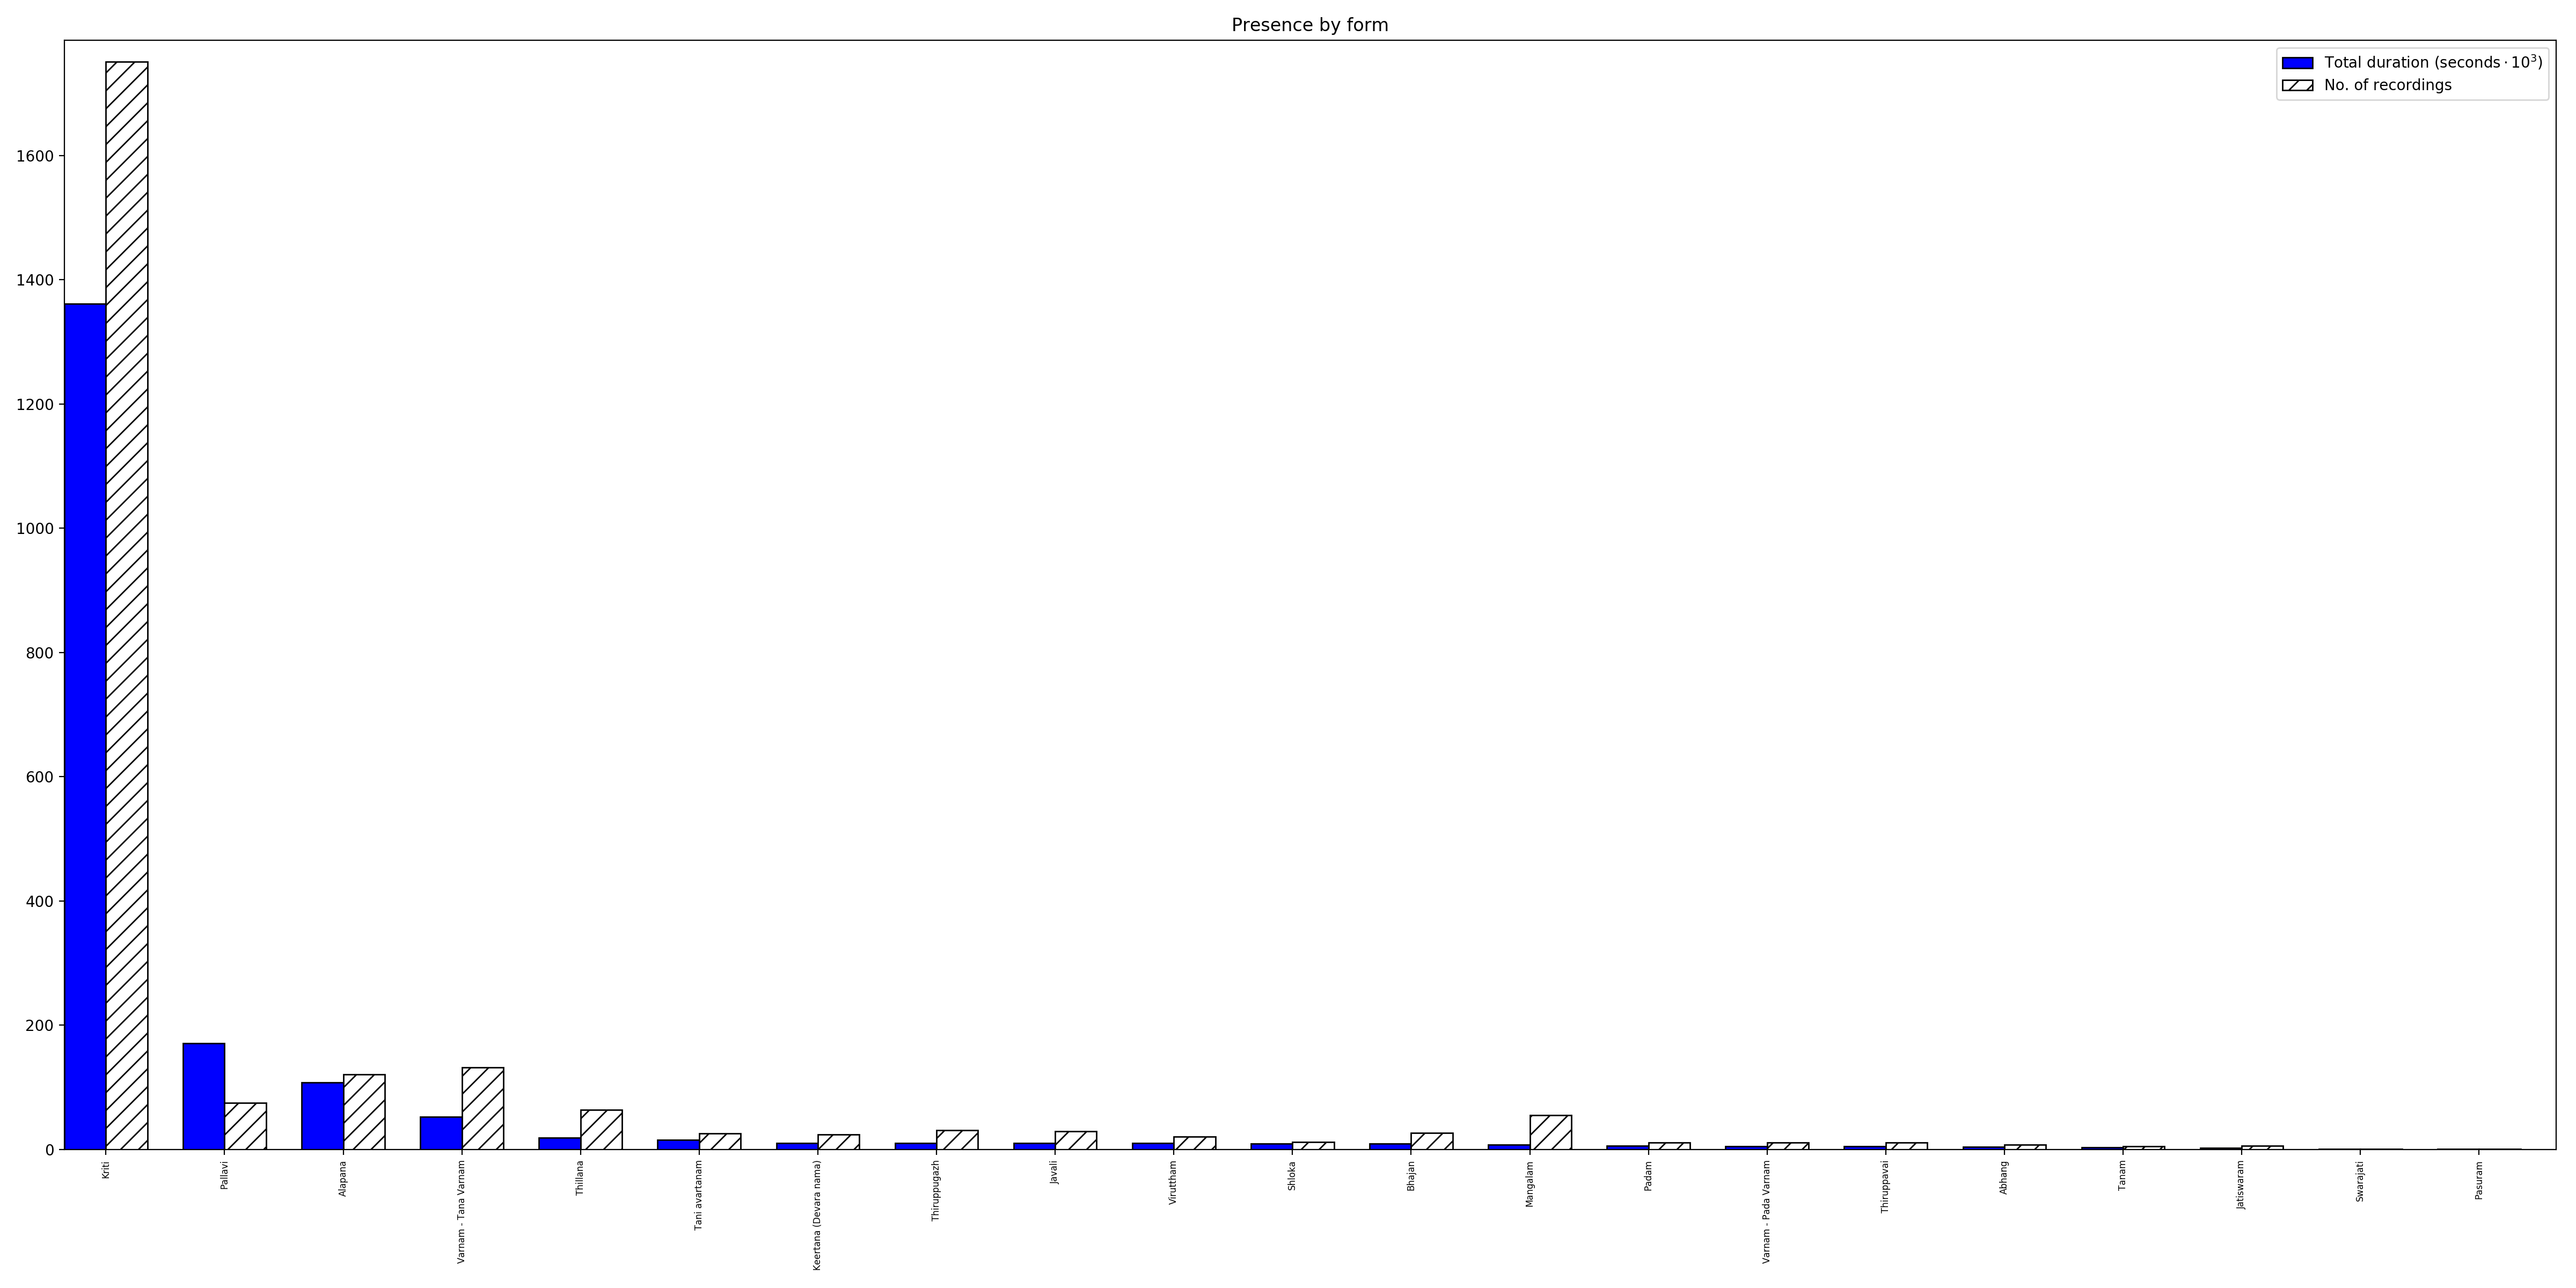
\includegraphics[scale=0.41]{histogram_form.png}
  \caption{The number and total duration of the recordings labeled with form.}
  % \label{fig:_}
\end{sidewaysfigure}

\begin{sidewaysfigure}%[h]
  % \hspace*{-0.6cm}
  \centering
  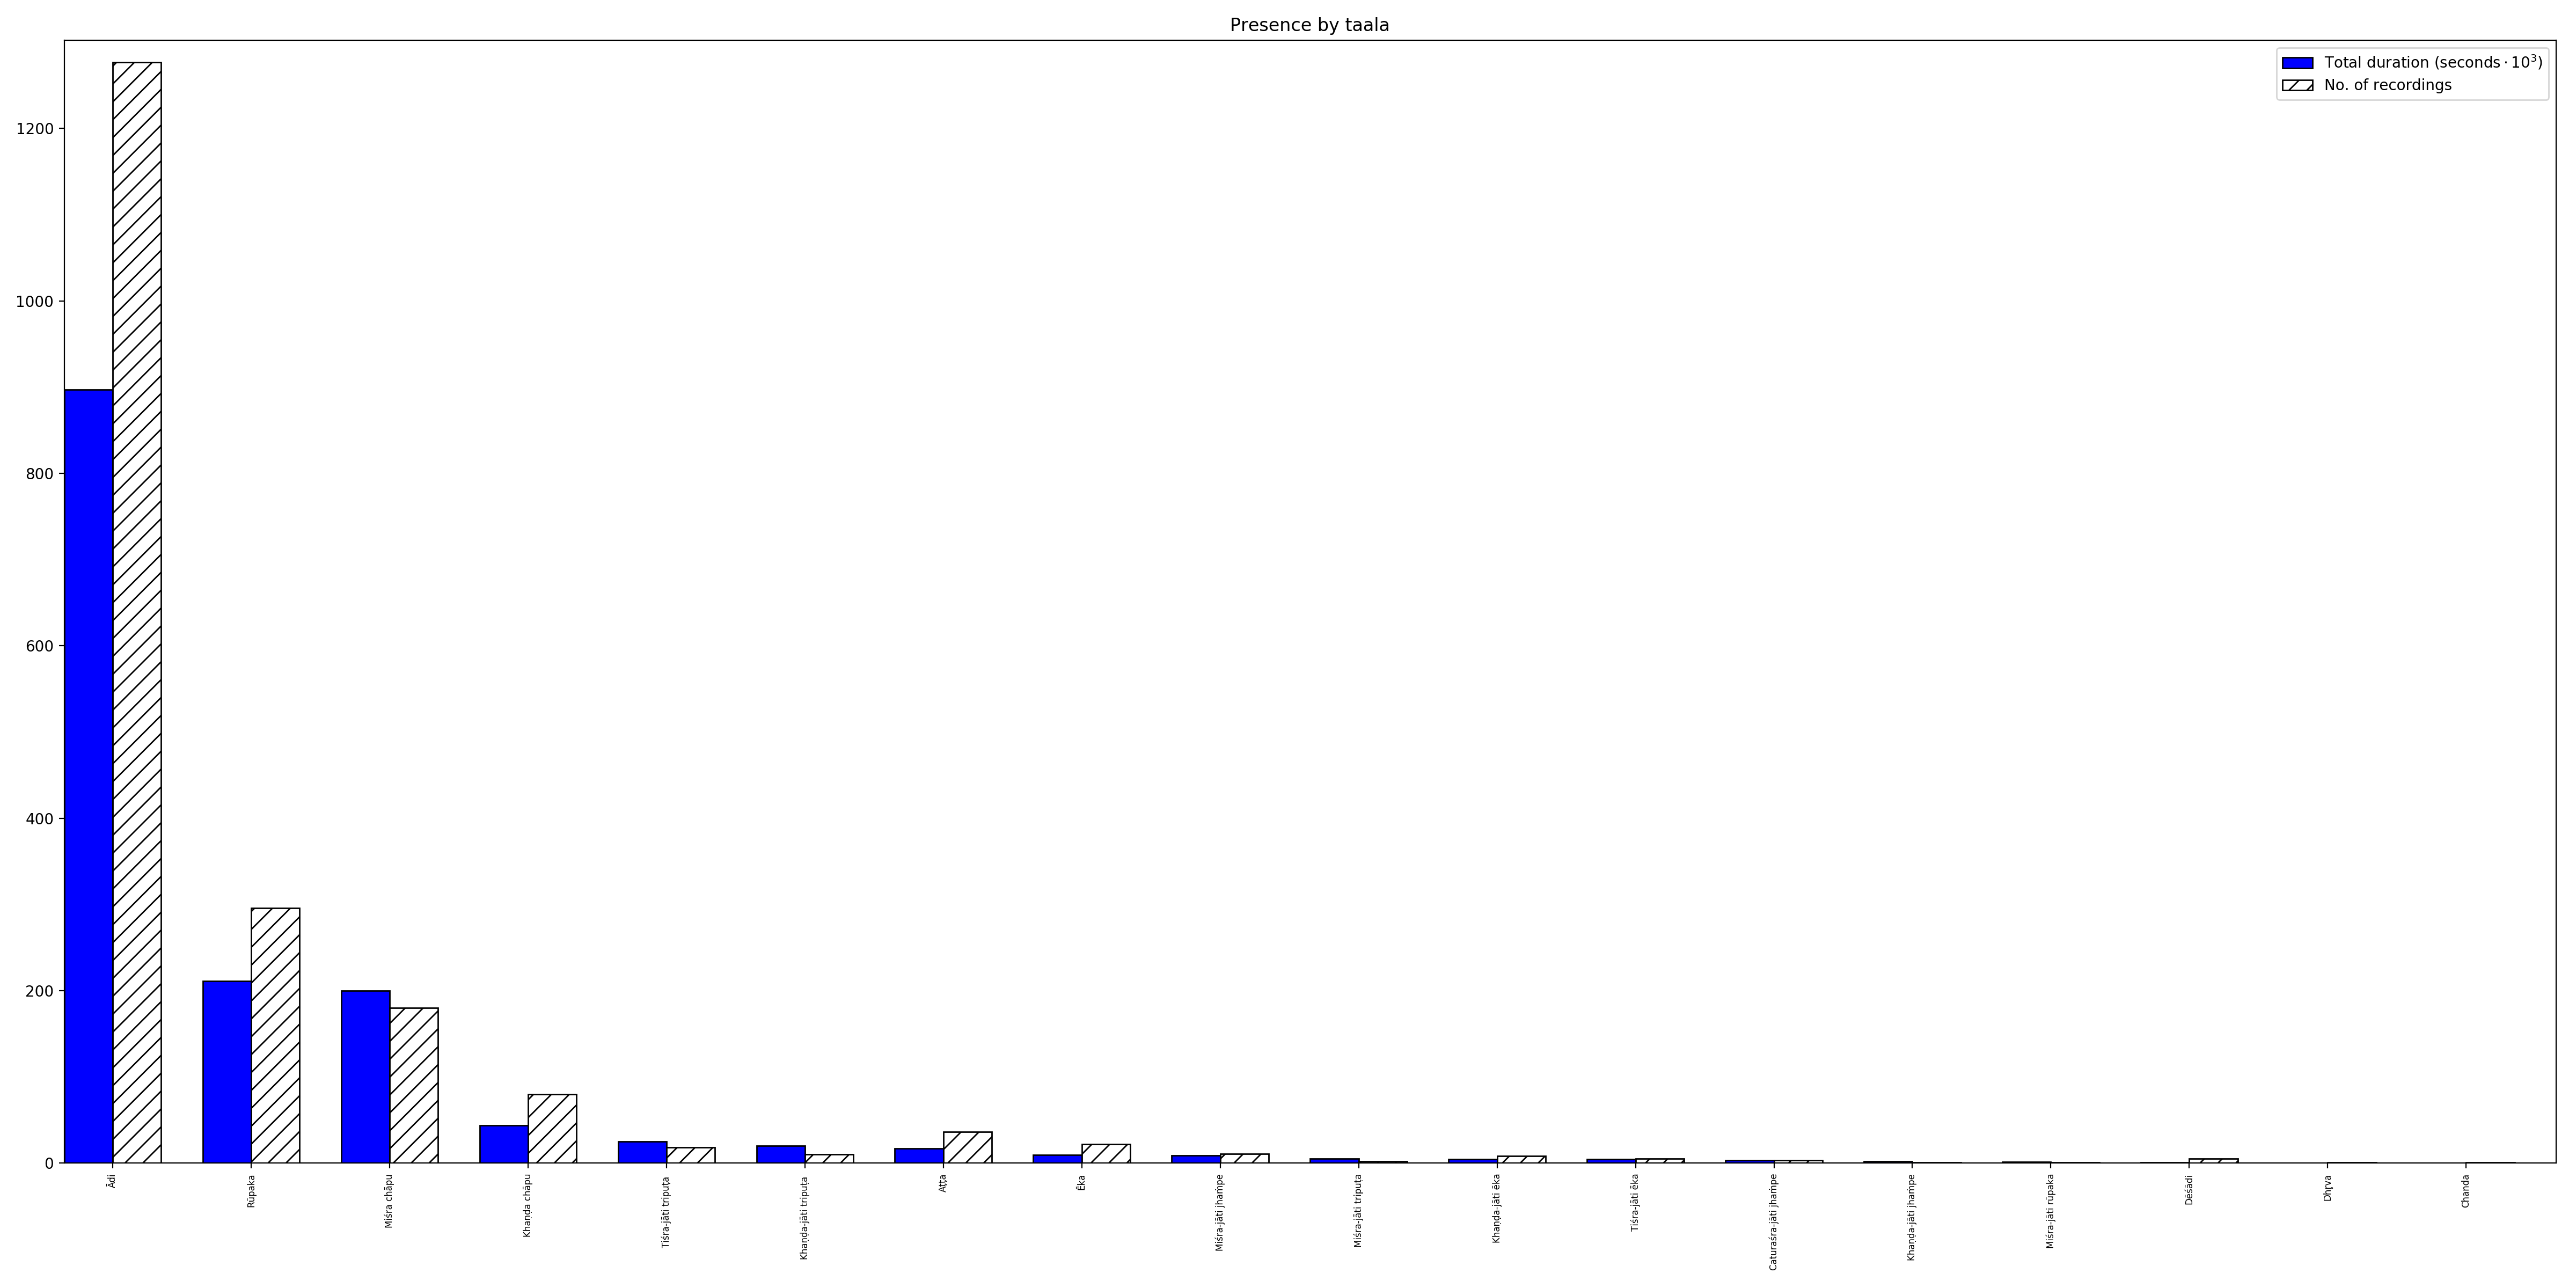
\includegraphics[scale=0.41]{histogram_taala.png}
  \caption{The number and total duration of the recordings labeled with t\=ala.}
  % \label{fig:_}
\end{sidewaysfigure}


\begin{sidewaysfigure}%[h]
  % \hspace*{-0.6cm}
  \centering
  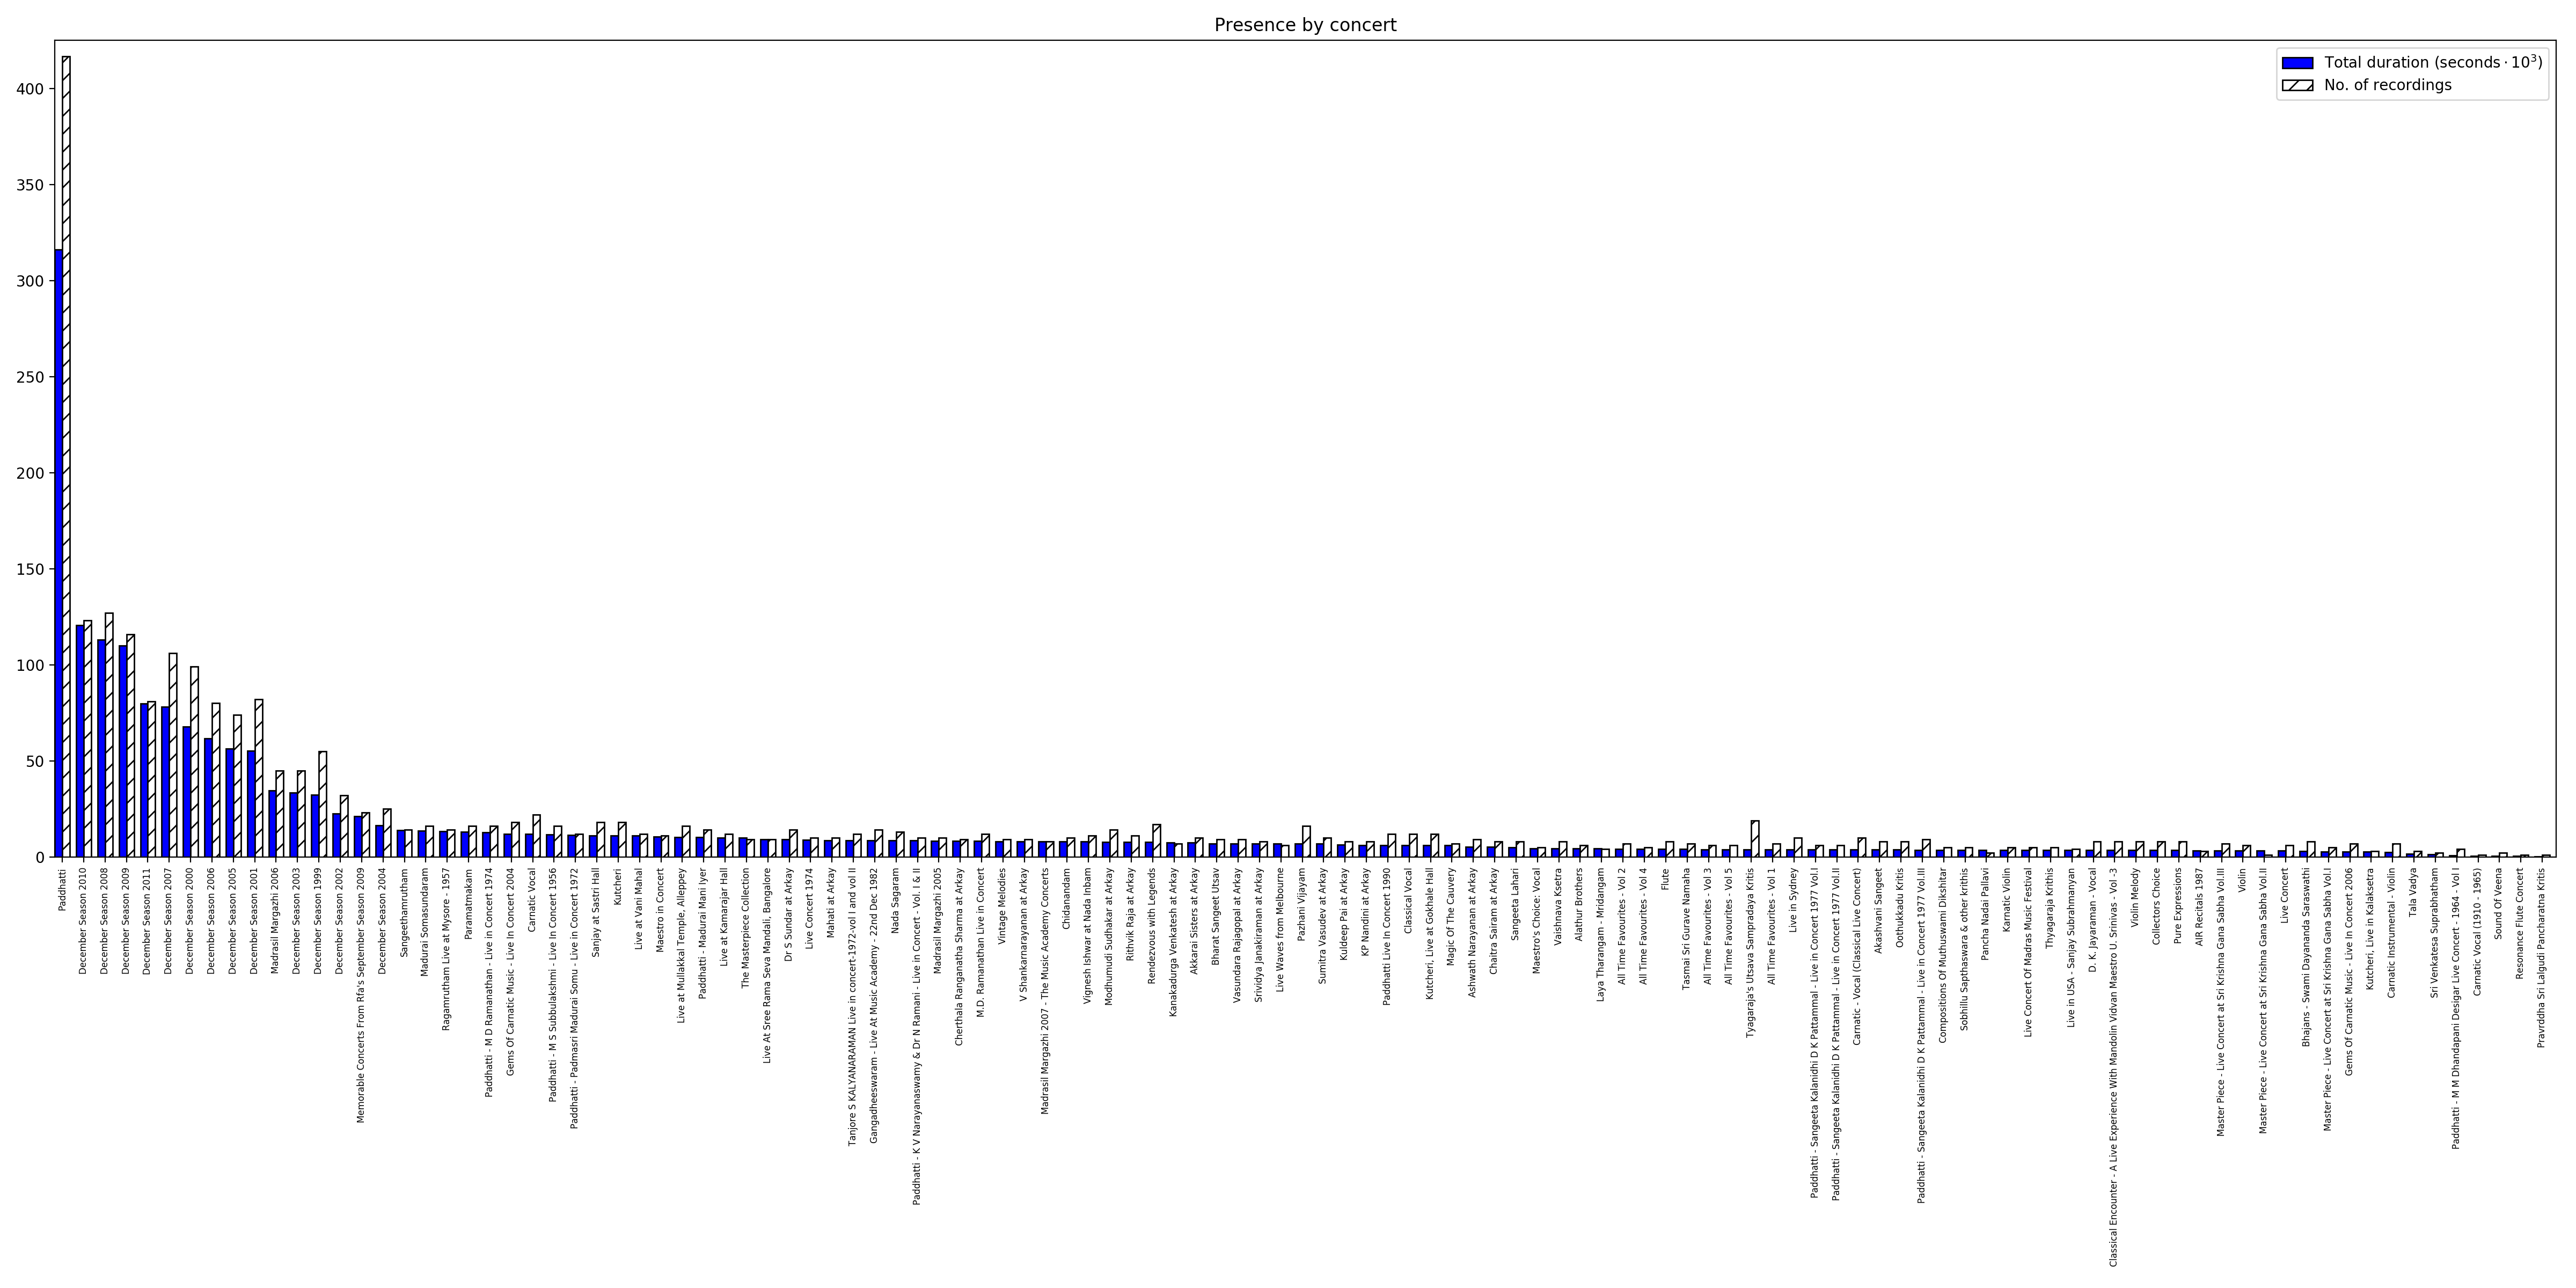
\includegraphics[scale=0.41]{histogram_concert.png}
  \caption{The number and total duration of the recordings labeled with concert.}
  % \label{fig:_}
\end{sidewaysfigure}

\begin{sidewaysfigure}%[h]
  % \hspace*{-0.6cm}
  \centering
  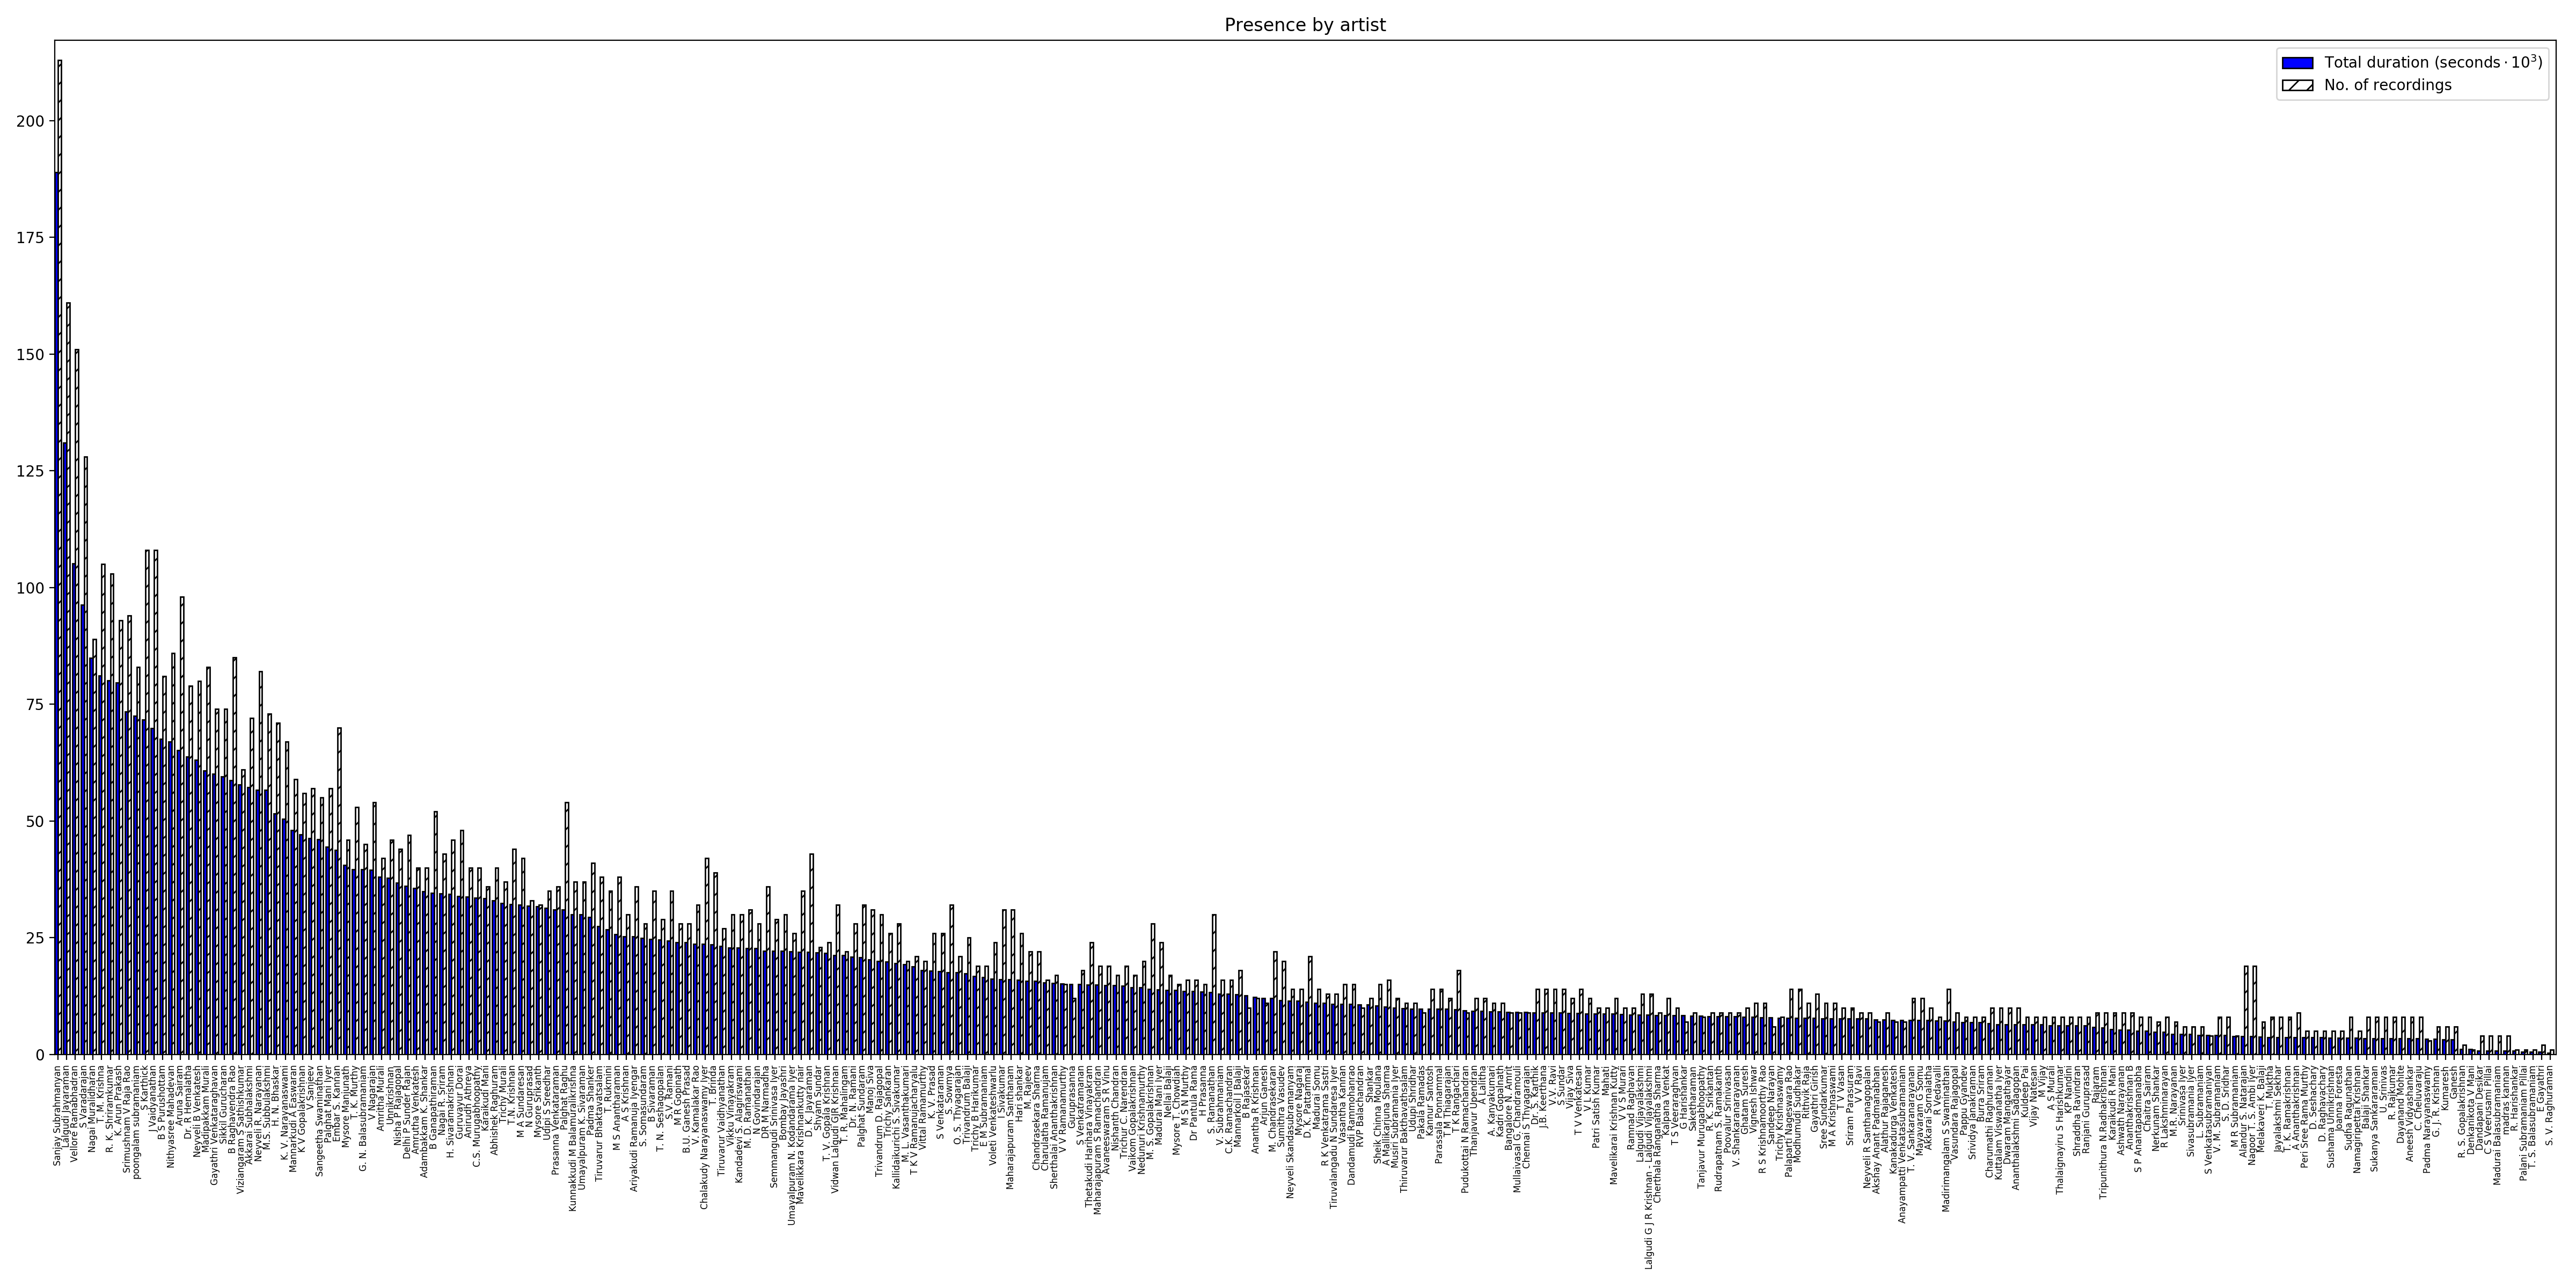
\includegraphics[scale=0.41]{histogram_artist.png}
  \caption{The number and total duration of the recordings labeled with artist.}
  % \label{fig:_}
\end{sidewaysfigure}


\begin{sidewaysfigure}%[h]
  % \hspace*{-0.6cm}
  \centering
  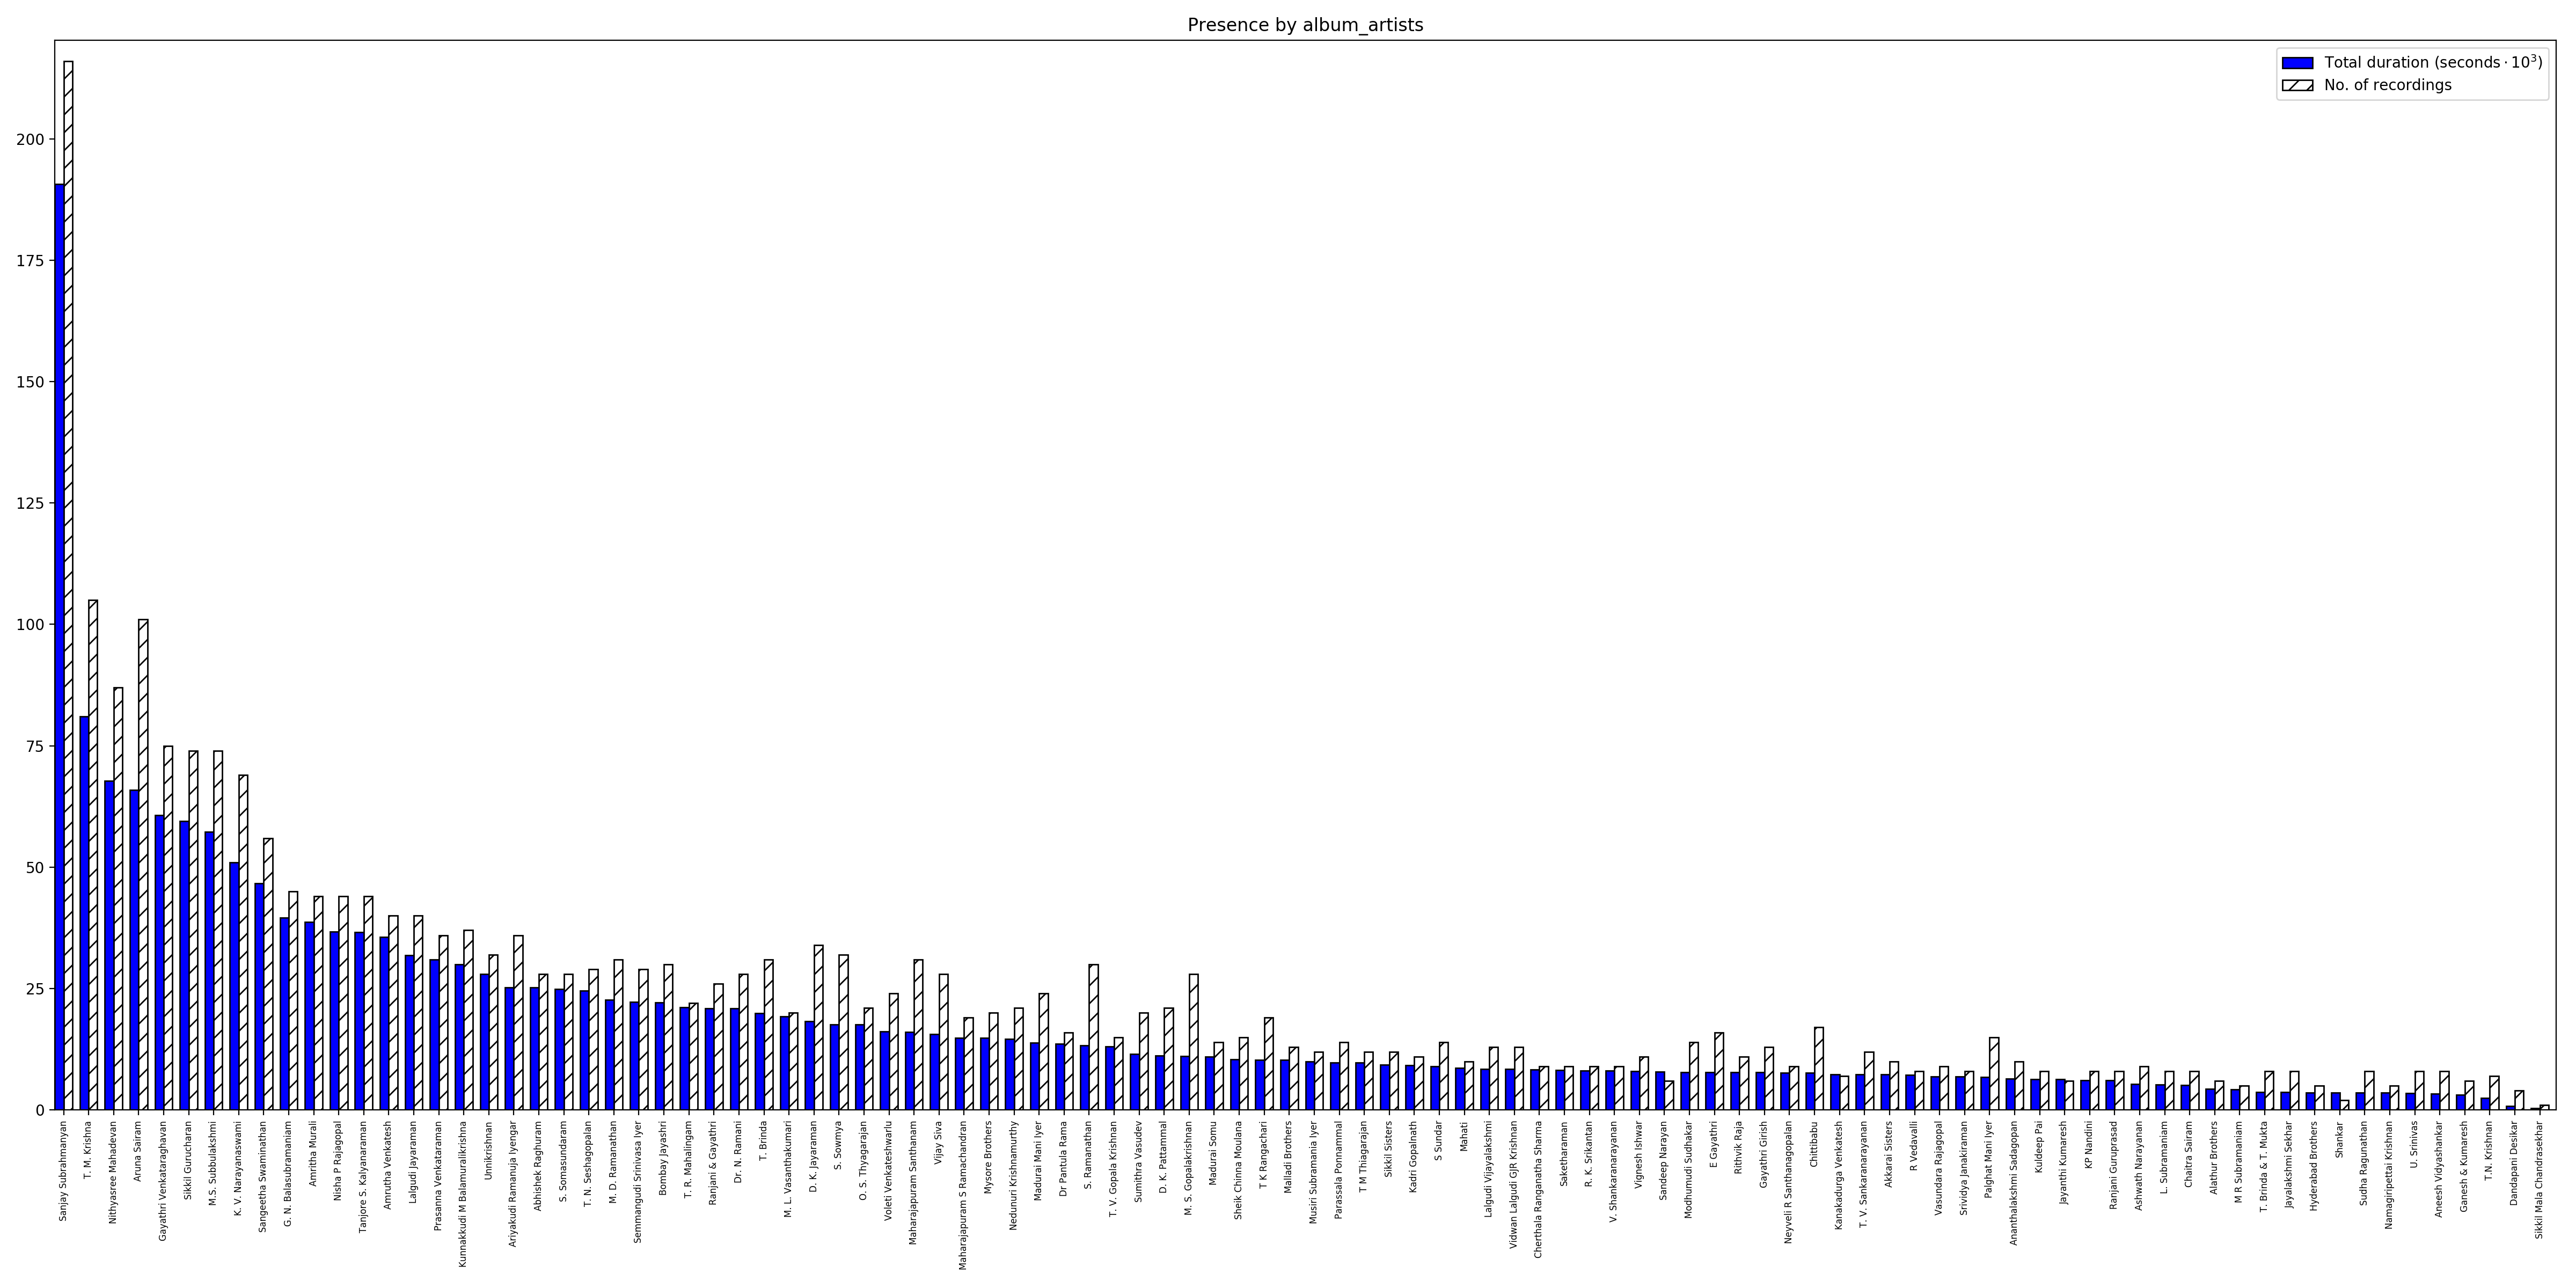
\includegraphics[scale=0.41]{histogram_album_artists.png}
  \caption{The number and total duration of the recordings labeled with album artist.}
  % \label{fig:_}
\end{sidewaysfigure}


\begin{sidewaysfigure}%[h]
  % \hspace*{-0.6cm}
  \centering
  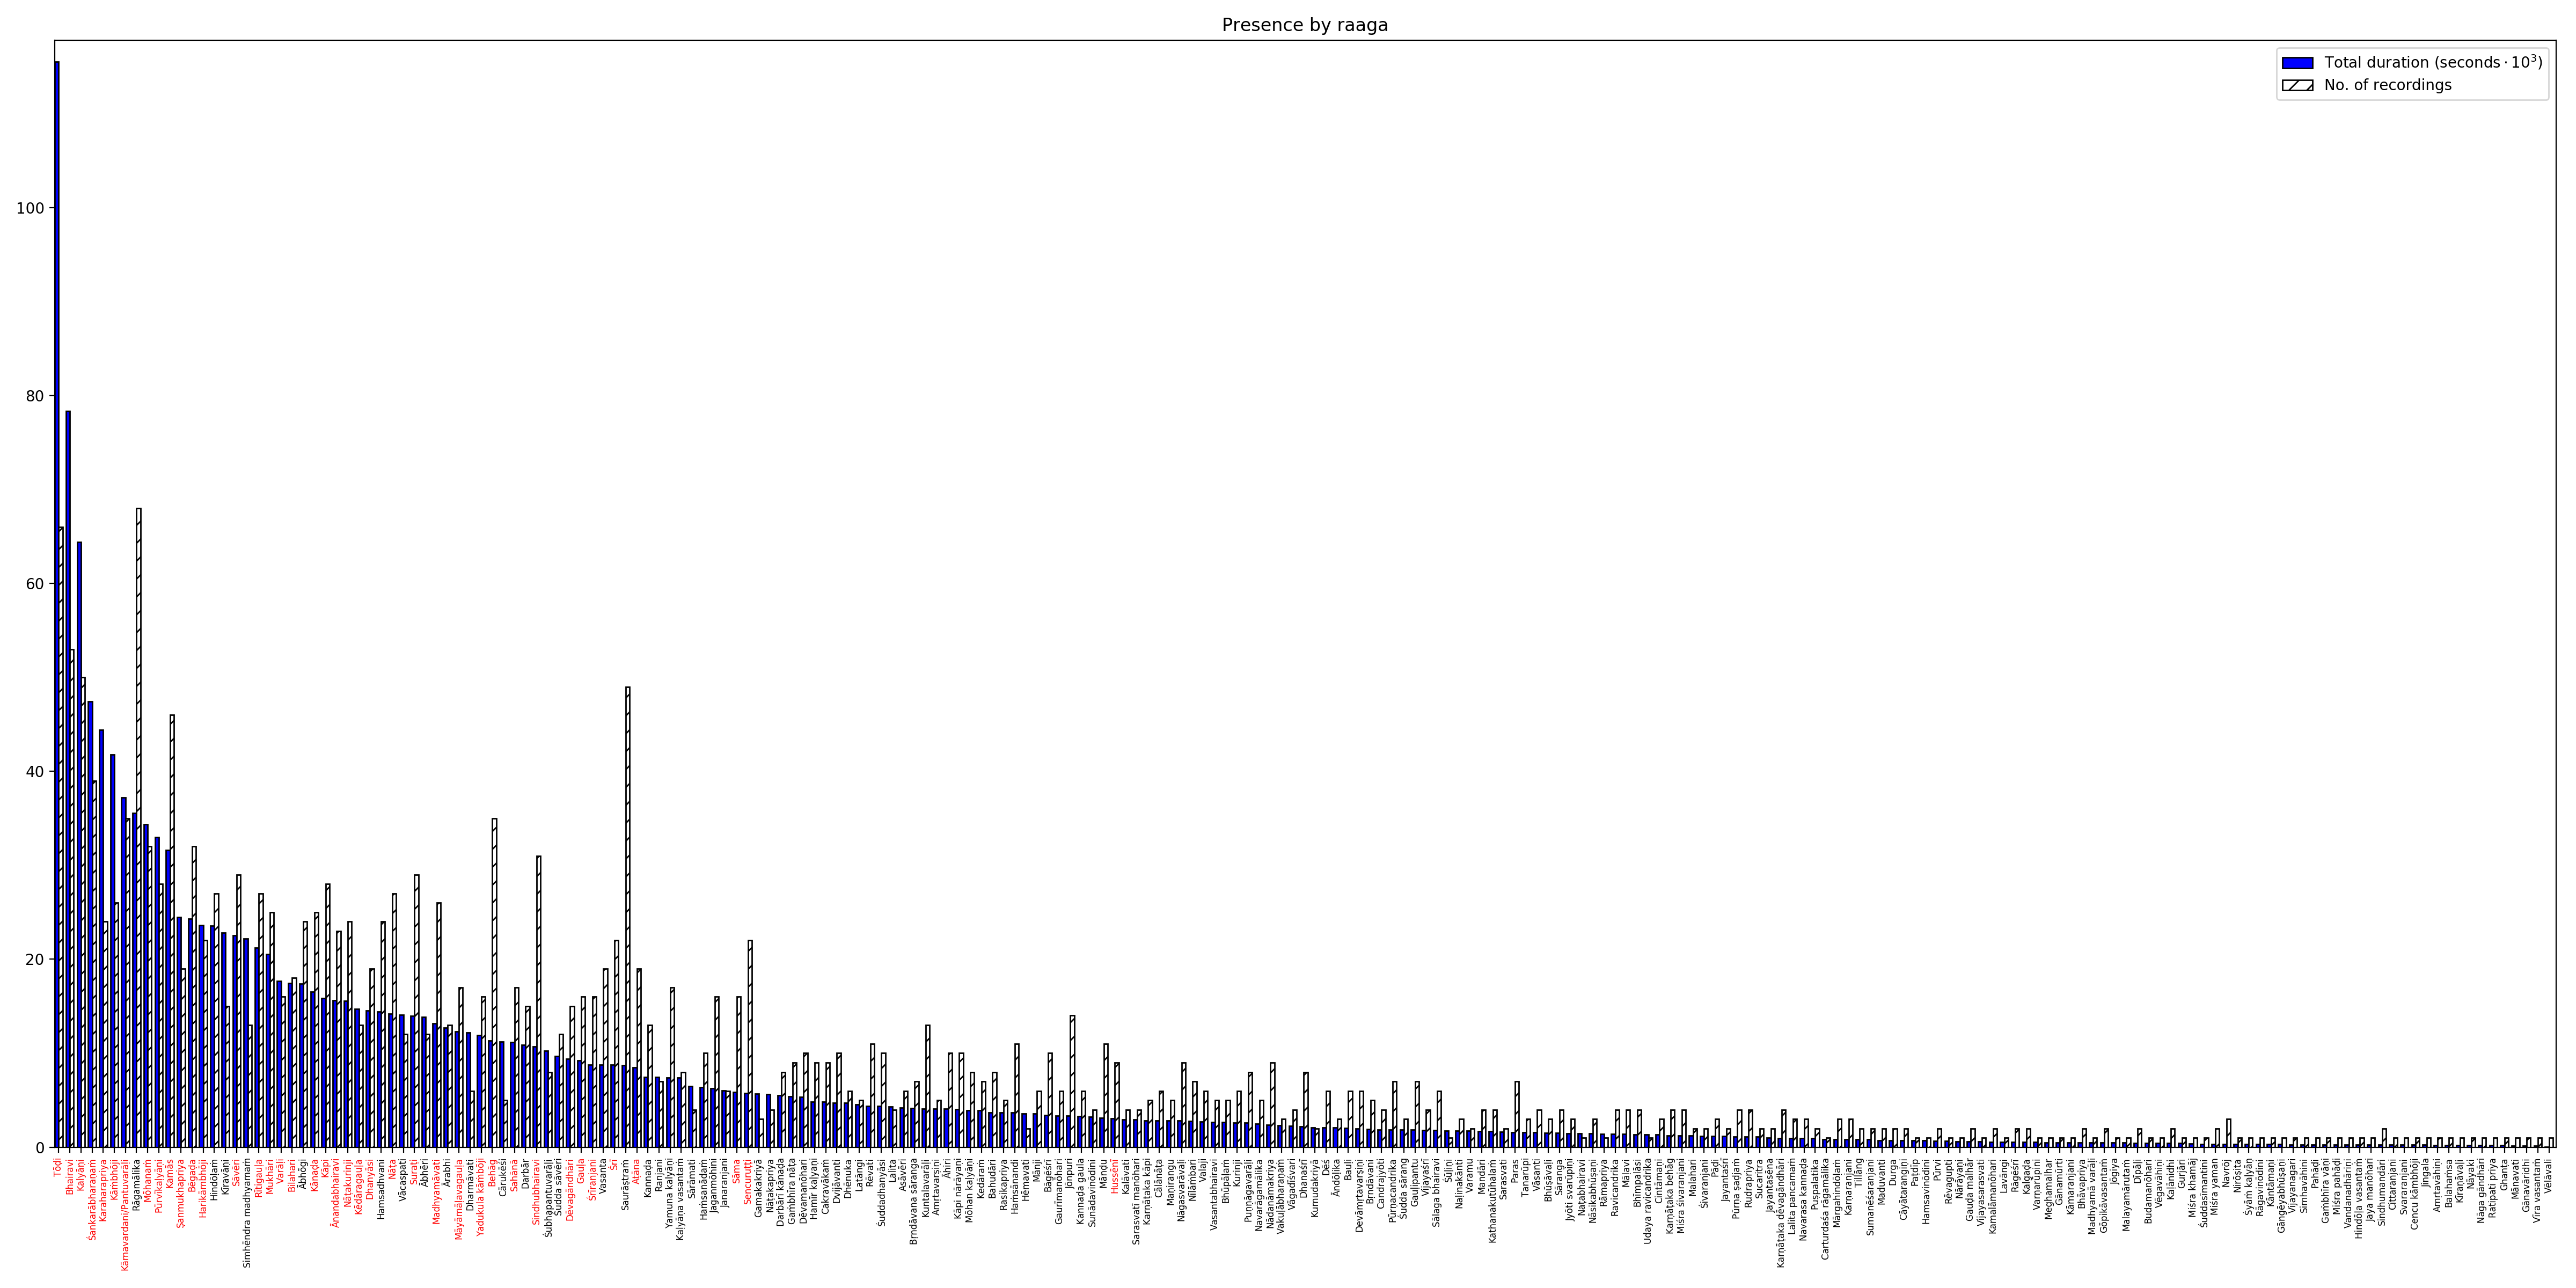
\includegraphics[scale=0.41]{histogram_raaga.png}
  \caption{The number and total duration of the recordings labeled with r\=aga. In red are the r\=agas present in Gulati's \(RRD_{CMD}\) test set.}
  % \label{fig:_}
\end{sidewaysfigure}


\begin{table}
  \centering
  \resizebox{\textwidth*7/8}{!}{%
    \begin{tabular}{*5c}\toprule
      \bfseries R\=aga & \bfseries \#Recordings & \bfseries Total duration & \bfseries Dur. in RRD_{CMD} & \bfseries Dur. in corpus\\\Midrule
      T\=o\d{d}i                       & 12 & 7h15m31s &      6.38\% &      12.15\%  \\\midrule
      Bhairavi                         & 12 & 5h18m19s &      4.66\% &      8.24\%  \\\midrule
      Kaly\=a\d{n}i                    & 11 & 5h17m19s &      4.65\% &      6.77\%  \\\midrule
      Śankar\=abhara\d{n}a\.{m}        & 10 & 3h42m47s &      3.26\% &      4.99\%  \\\midrule
      Karaharapriya                    & 11 & 6h42m03s &      5.89\% &      4.67\%  \\\midrule
      K\=a\.{m}bh\=oji                 & 10 & 5h19m24s &      4.68\% &      4.39\%  \\\midrule
      K\=amavardani                    & 12 & 3h30m49s &      3.09\% &      3.91\%  \\\midrule
      M\=ohana\.{m}                    & 12 & 4h40m04s &      4.10\% &      3.61\%  \\\midrule
      P\=urv\={\i}ka\d{l}y\=a\d{n}i    & 12 & 5h51m54s &      5.15\% &      3.47\%  \\\midrule
      Kam\=as                          & 11 & 2h13m00s &      1.95\% &      3.33\%  \\\midrule
      \d{S}anmukhapriya                & 12 & 2h59m15s &      2.63\% &      2.58\%  \\\midrule
      B\=ega\d{d}a                     & 12 & 2h51m39s &      2.51\% &      2.56\%  \\\midrule
      Harik\=ambh\=oji                 & 11 & 3h57m57s &      3.49\% &      2.49\%  \\\midrule
      S\=av\=eri                       & 10 & 2h23m58s &      2.11\% &      2.37\%  \\\midrule
      R\={\i}tigau\d{l}a               & 12 & 3h13m50s &      2.84\% &      2.23\%  \\\midrule
      Mukh\=ari                        & 12 & 3h17m55s &      2.90\% &      2.16\%  \\\midrule
      Var\=a\d{l}i                     & 9  & 2h56m58s &      2.59\% &      1.86\% \\\midrule
      Bilahari                         & 10 & 3h05m57s &      2.72\% &      1.83\%  \\\midrule
      K\=ana\d{d}a                     & 11 & 2h43m42s &      2.40\% &      1.74\%  \\\midrule
      K\=api                           & 11 & 1h05m28s &      0.96\% &      1.67\%  \\\midrule
      \=Anandabhairavi                 & 11 & 1h42m04s &      1.50\% &      1.64\%  \\\midrule
      N\=a\d{t}akurinji                & 12 & 1h45m13s &      1.54\% &      1.64\%  \\\midrule
      K\=ed\=aragau\d{l}a              & 11 & 3h58m17s &      3.49\% &      1.55\%  \\\midrule
      Dhany\=asi                       & 11 & 2h24m28s &      2.12\% &      1.53\%  \\\midrule
      N\=a\d{t}a                       & 11 & 1h37m13s &      1.42\% &      1.49\%  \\\midrule
      Sura\d{t}i                       & 12 & 2h17m57s &      2.02\% &      1.47\%  \\\midrule
      Madhyam\=avati                   & 10 & 2h15m56s &      1.99\% &      1.39\%  \\\midrule
      M\=ay\=am\=a\d{l}avagau\d{l}a    & 10 & 2h06m07s &      1.85\% &      1.30\%  \\\midrule
      Yaduku\.{l}a k\=a\.{m}b\=oji     & 10 & 1h53m48s &      1.67\% &      1.26\%  \\\midrule
      Beh\=ag                          & 12 & 1h12m59s &      1.07\% &      1.19\%  \\\midrule
      Sah\=an\=a                       & 11 & 2h30m08s &      2.20\% &      1.18\%  \\\midrule
      Sindhubhairavi                   & 12 & 1h01m05s &      0.89\% &      1.12\%  \\\midrule
      D\=evag\=andh\=ari               & 12 & 2h13m36s &      1.96\% &      0.99\%  \\\midrule
      Gau\d{l}a                        & 12 & 2h00m09s &      1.76\% &      0.97\%  \\\midrule
      Śr\={\i}ranjani                  & 9  & 1h19m32s &      1.17\% &      0.92\% \\\midrule
      Śr\={\i}                         & 9  & 0h52m09s &      0.76\% &      0.92\% \\\midrule
      A\d{t}\=ana                      & 11 & 1h35m05s &      1.39\% &      0.89\%  \\\midrule
      S\=ama                           & 10 & 0h55m48s &      0.82\% &      0.62\%  \\\midrule
      Sencuru\d{t}\d{t}i               & 12 & 0h53m35s &      0.78\% &      0.60\%  \\\midrule
      Huss\=en\={\i}                   & 8  & 0h43m18s &      0.63\% &      0.32\%  \\\bottomrule
  \end{tabular}}
  \caption{The number of recordings and total duration for each of the 40 r\=agas present in Gulati's \(RRD_{CMD}\) test set that were found in the Dunya database, as well as their relative durations with respect to the \(RRD_{CMD}\) dataset and the whole downloaded carnatic corpus.}
  \label{fig:rrd-stats}
\end{table}
